\begin{figure}[H]
\centering
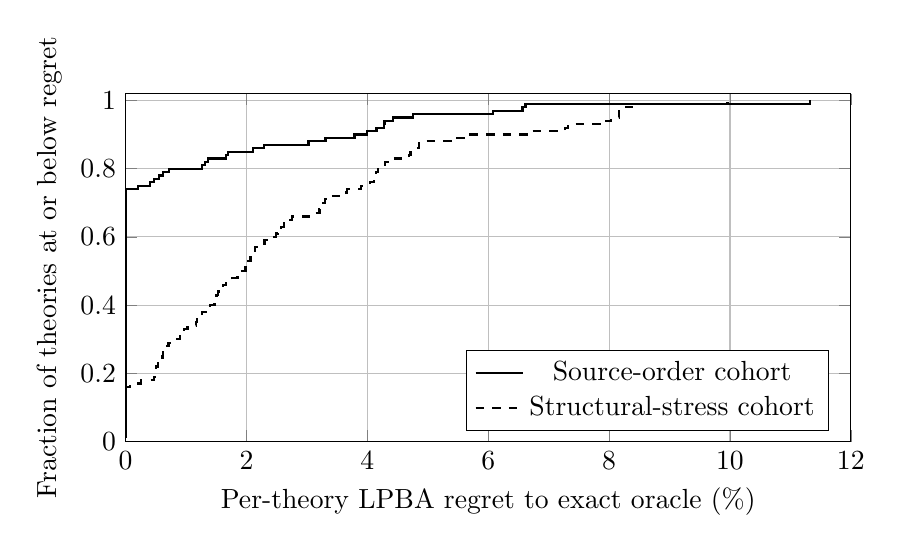
\begin{tikzpicture}
\begin{axis}[width=.89\textwidth,height=6.0cm,xlabel={Per-theory LPBA regret to exact oracle (\%)},ylabel={Fraction of theories at or below regret},xmin=0,xmax=12,ymin=0,ymax=1.02,grid=major,legend pos=south east]
\addplot+[black,mark=none,thick,const plot] coordinates {(0.000,0.010) (0.000,0.020) (0.000,0.030) (0.000,0.040) (0.000,0.050) (0.000,0.060) (0.000,0.070) (0.000,0.080) (0.000,0.090) (0.000,0.100) (0.000,0.110) (0.000,0.120) (0.000,0.130) (0.000,0.140) (0.000,0.150) (0.000,0.160) (0.000,0.170) (0.000,0.180) (0.000,0.190) (0.000,0.200) (0.000,0.210) (0.000,0.220) (0.000,0.230) (0.000,0.240) (0.000,0.250) (0.000,0.260) (0.000,0.270) (0.000,0.280) (0.000,0.290) (0.000,0.300) (0.000,0.310) (0.000,0.320) (0.000,0.330) (0.000,0.340) (0.000,0.350) (0.000,0.360) (0.000,0.370) (0.000,0.380) (0.000,0.390) (0.000,0.400) (0.000,0.410) (0.000,0.420) (0.000,0.430) (0.000,0.440) (0.000,0.450) (0.000,0.460) (0.000,0.470) (0.000,0.480) (0.000,0.490) (0.000,0.500) (0.000,0.510) (0.000,0.520) (0.000,0.530) (0.000,0.540) (0.000,0.550) (0.000,0.560) (0.000,0.570) (0.000,0.580) (0.000,0.590) (0.000,0.600) (0.000,0.610) (0.000,0.620) (0.000,0.630) (0.000,0.640) (0.000,0.650) (0.000,0.660) (0.000,0.670) (0.000,0.680) (0.000,0.690) (0.000,0.700) (0.000,0.710) (0.000,0.720) (0.000,0.730) (0.000,0.740) (0.211,0.750) (0.409,0.760) (0.473,0.770) (0.546,0.780) (0.613,0.790) (0.722,0.800) (1.263,0.810) (1.312,0.820) (1.363,0.830) (1.664,0.840) (1.700,0.850) (2.111,0.860) (2.290,0.870) (3.026,0.880) (3.306,0.890) (3.786,0.900) (3.996,0.910) (4.150,0.920) (4.275,0.930) (4.284,0.940) (4.425,0.950) (4.753,0.960) (6.078,0.970) (6.566,0.980) (6.617,0.990) (11.326,1.000)};
\addlegendentry{Source-order cohort}
\addplot+[black,dashed,mark=none,thick,const plot] coordinates {(0.000,0.010) (0.000,0.020) (0.000,0.030) (0.000,0.040) (0.000,0.050) (0.000,0.060) (0.000,0.070) (0.000,0.080) (0.000,0.090) (0.000,0.100) (0.000,0.110) (0.000,0.120) (0.000,0.130) (0.000,0.140) (0.000,0.150) (0.000,0.160) (0.076,0.170) (0.250,0.180) (0.468,0.190) (0.480,0.200) (0.502,0.210) (0.504,0.220) (0.530,0.230) (0.567,0.240) (0.611,0.250) (0.620,0.260) (0.622,0.270) (0.643,0.280) (0.711,0.290) (0.769,0.300) (0.900,0.310) (0.942,0.320) (0.967,0.330) (1.024,0.340) (1.166,0.350) (1.176,0.360) (1.236,0.370) (1.262,0.380) (1.347,0.390) (1.396,0.400) (1.471,0.410) (1.486,0.420) (1.504,0.430) (1.532,0.440) (1.610,0.450) (1.616,0.460) (1.667,0.470) (1.768,0.480) (1.850,0.490) (1.870,0.500) (1.985,0.510) (1.997,0.520) (2.020,0.530) (2.066,0.540) (2.092,0.550) (2.138,0.560) (2.139,0.570) (2.202,0.580) (2.299,0.590) (2.400,0.600) (2.490,0.610) (2.520,0.620) (2.577,0.630) (2.615,0.640) (2.679,0.650) (2.748,0.660) (3.037,0.670) (3.207,0.680) (3.214,0.690) (3.226,0.700) (3.295,0.710) (3.409,0.720) (3.654,0.730) (3.666,0.740) (3.893,0.750) (4.038,0.760) (4.111,0.770) (4.129,0.780) (4.144,0.790) (4.179,0.800) (4.245,0.810) (4.297,0.820) (4.399,0.830) (4.692,0.840) (4.713,0.850) (4.746,0.860) (4.859,0.870) (4.859,0.880) (5.426,0.890) (5.698,0.900) (6.696,0.910) (7.267,0.920) (7.320,0.930) (7.955,0.940) (8.037,0.950) (8.165,0.960) (8.169,0.970) (8.211,0.980) (8.413,0.990) (9.960,1.000)};
\addlegendentry{Structural-stress cohort}
\end{axis}
\end{tikzpicture}
\caption{Empirical distribution across independent theories within each nonoverlapping cohort. A point at zero means LPBA matches the exact whole-order value; the structural-stress cohort was selected on support structure, not sampled as a population estimate.\label{fig:regret}}
\end{figure}
